\documentclass[12pt]{article}
\usepackage{graphicx}
\usepackage[]{mcode}
\usepackage{amsmath}
\usepackage[T1]{fontenc}
%\usepackage{lingmacros}
%\usepackage{tree-dvips}
%\usepackage{blindtext}
%\usepackage[utf8]{inputenc}

\begin{document}

\title{CMSC 460 - HW2}
\author{Gudjon Einar Magnusson}

\maketitle

\section{Matrix Vector Product}

\subsection{MatVecProd\_a}
\begin{minipage}{\linewidth}
\lstinputlisting{../MatVecProd_a.m}
\end{minipage}


\subsection{MatVecProd\_b}
\begin{minipage}{\linewidth}
\lstinputlisting{../MatVecProd_b.m}
\end{minipage}

\subsection{MatVecProd\_c}
\begin{minipage}{\linewidth}
\lstinputlisting{../MatVecProd_c.m}
\end{minipage}

\subsection{MatVecProd\_d}
\begin{minipage}{\linewidth}
\lstinputlisting{../MatVecProd_d.m}
\end{minipage}

\subsection{Evaluation}

To compare the different implementations I measured the time it took to calculate a matrix vector product for square matrices of different sizes. For each implementation I tested a matrix of size 128, 256, 512,1024, 2048 and 4096. Figure \ref{fig_matVecProdPlot} shows the result. We can see that the column-major implementations (a and c) are consistently faster than the row-major counter part. We can also see that the vectorized implementations (d and c) get an even greater speed boost. Finally we see that the built in Matlab operator is by far the fastest.

By indexing the matrix in column-major order we gain the benefit of memory proximity and optimal cache hits. This is a noticeable improvement but not as noticeable as changing to a vectorized implementation. By doing that we gain the benefit of the optimization that has been built in by the designers of Matlab. This is even more obvious when looking at the superior speed of the * operator.

\begin{figure}
	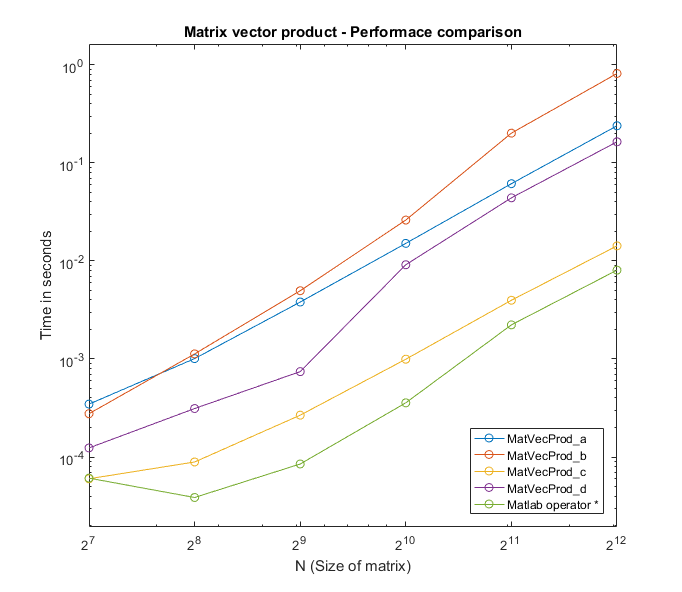
\includegraphics[width=\linewidth]{matVecProdPlot}
	\centering
	\label{fig_matVecProdPlot}
\end{figure}

\section{}

See step by step solution in appendix.

\[
L =  
\begin{bmatrix}
    1 & 0 & 0  \\
    \frac{1}{3} & 1 & 0 \\
    \frac{1}{6} & \frac{5}{14} & 1
\end{bmatrix}
\\
U =  
\begin{bmatrix}
    -6 & 3 & -15  \\
    0 & -7 & 3 \\
    0 & 0 & -14
\end{bmatrix}
\\
P =  
\begin{bmatrix}
    0 & 0 & 1 \\
    0 & 1 & 0 \\
    1 & 0 & 1
\end{bmatrix}
\\
x =  
\begin{bmatrix}
    3  \\
    -1 \\
    -2 
\end{bmatrix}
\]

This answer matches what the \textit{lu} function returns, except that L is flipped horizontally. This is just a matter of notation.


\section{} %%Problem 3

Only thing added to the \textit{lutx} function is a line to initialize \textit{sig} as 1 and a line to flip the sign of \textit{sig} every time a row is swapped.

\begin{minipage}{\linewidth}
\lstinputlisting{../lutx.m}
\end{minipage}

\textit{mydet} gets the determinant of $U$ by computing the product of its diagonal elements and to get the determinant of $A$ it multiplies by \textit{sig}.

\begin{minipage}{\linewidth}
\lstinputlisting{../mydet.m}
\end{minipage}

To verify than my implementation works I used the following script:

\begin{minipage}{\linewidth}
\lstinputlisting{../prob3.m}
\end{minipage}

\section{} %%Problem 4

To measure the performance of each implementation I tested what order matrix it could solve in 10 seconds. To do this I ran the function repeatedly and increased the size of the matrix in increments of 50. Smaller increments would have given a more accurate result but took longer than I was willing to wait.

\begin{description}
	\item[explutx] \hfill \\
	Solved a Matrix of size 1150 in 11.26s
	\item[lutx] \hfill \\
	Solved a Matrix of size 1500 in 10.31s
	\item[lu] \hfill \\
	Solved a Matrix of size 12800 in 10.06s
\end{description}

As you can see the built in \textit{lu} function is by far the fastest, it can handle a order of magnitude larger matrix in the same time as the home brew functions. Using the vectorized implementation gives a noticeable boost but nothing major.

\begin{minipage}{\linewidth}
\lstinputlisting{../explutx.m}
\end{minipage}

To verify than my implementation works I used the following script:

\begin{minipage}{\linewidth}
\lstinputlisting{../test_prob4.m}
\end{minipage}


\section{} %%Problem 5

\textit{myinv} finds the inverse of a matrix by solving $Ax_j = e_j$ where $x_j$ is the j-th column of the inverse matrix and $e_j$ is the j-th column of the identity matrix.

\begin{minipage}{\linewidth}
\lstinputlisting{../myinv.m}
\end{minipage}

To verify than my implementation works I used a similar script as before. Omitted to save paper.

\end{document}